\documentclass[../ECE459FinalProjectReport.tex]{subfiles}
\begin{document}
\chapter{Methodology}
This chapter presents the methodology and the relevant theories employed in the project. The simulations were executed within the Jupyter Notebook environment, leveraging essential packages for numerical computation, signal analysis, and plotting, namely \verb|numpy|, \verb|scipy|, and \verb|matplotlib|.

\section{Determination of Signal Bandwidth}
It is of significance to measure the bandwidth of message signals. As is stated in \cite[Sec. 7.2.3]{kudekiAnalogSignalsSystems2009} and illustrated in Figure \ref{fig:bw}, the bandwidth $B_W$ of a band-limited signal is the minimum frequency component that the signal has almost zero magnitude at any $f>B_W$, which means
\begin{equation}\label{eq:bw-def}
    S\left( f \right) =
    \begin{cases}
        \napprox 0, & \text{for} \left| f \right|=B_W      \\
        \approx 0,  & \text{for any }\left| f \right| >B_W \\
    \end{cases}.
\end{equation}
In the experiment, the bandwidth of a band-limited signal can be determined by visually observing the spectrum or by calculating the maximum frequency with non-zero frequency response.
\begin{figure}[tb]
    \centering
    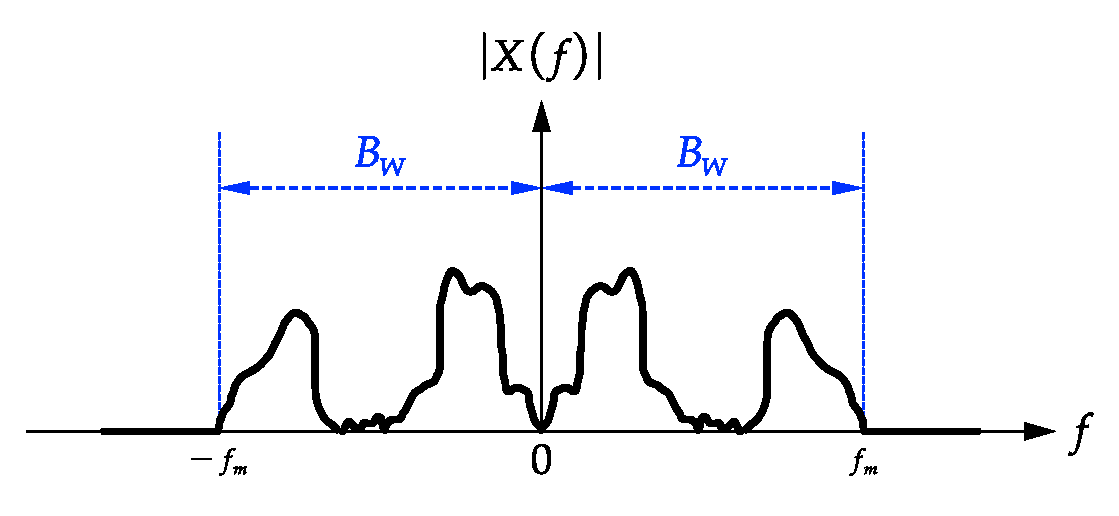
\includegraphics[scale=.5]{plots/bw.pdf}
    \caption{The bandwidth of the signal is $B_W$.}
    \label{fig:bw}
\end{figure}

\section{Additive White Gaussian Noise}
Additive White Gaussian Noise (AWGN) refers to a Gaussian process that can be directly added to a signal to approximate a noise-distorted signal in a real-life communication channel.

A Gaussian process denoted as $\mathrm{N}\left[ \mu, \sigma^2 \right]$ has the probability density function as
\begin{equation}
    f_{Gaussian}\left(u\right) = \frac{1}{\sqrt{2\pi\sigma^2}}\exp\left[ -\frac{\left(u-v\right)^2}{2\sigma^2} \right].
\end{equation}
It has mean $\mu$ and standard deviation $\sigma^2$.

According to \cite[Sec. 8.10]{haykinIntroductionAnalogDigital2007}, a noise process is called white noise if it has zero-mean and its power spectral density satisfies
\begin{equation}
    S_W\left(f\right) = \frac{N_0}{2}.
\end{equation}
The power spectrum of a Python-generated white Gaussian noise process is shown in Figure \ref{fig:white-noise-spectrum}.
\begin{figure}[tb]
    \centering
    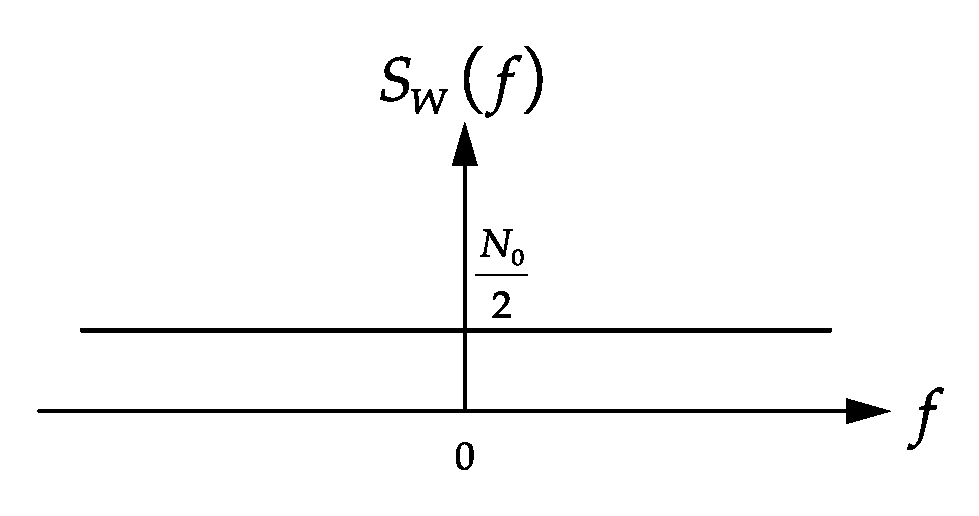
\includegraphics[scale=0.35]{plots/white-noise-power-spectrum.pdf}
    \caption{The power spectrum of a white noise process.}
    \label{fig:white-noise-spectrum}
\end{figure}

In this project, the AWGN process will be simulated using \verb|numpy.random.normal()| function. Figure \ref{fig:gaussian-noise} shows a Python-generated Gaussian noise process and its frequency spectrum.
\begin{figure}[tb]
        \centering
        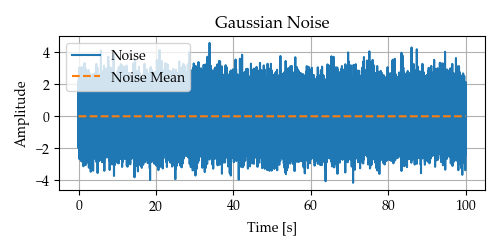
\includegraphics[width=0.6\linewidth]{plots/gaussian_noise.png}
        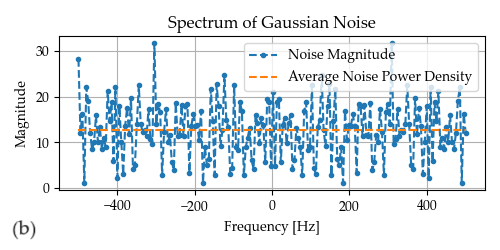
\includegraphics[width=0.6\linewidth]{plots/gaussian_noise_spectrum.png}
        \caption{The Python-generated Gaussian process $\mathrm{N}\left[\mu = 0, \sigma^2 = 1\right]$ and its spectrum.}
        \label{fig:gaussian-noise}
\end{figure}


\section{AM Simulation}
\subsection{Envelope Modulation}
%?? What about transmission bandwidth??
Consider a message signal $m\left(t\right)$ and carrier wave $A_c \cos\left(2\pi f_c t + \phi\right)$ where $\phi$ is the phase delay of the local oscillator. In this project, we pick $\phi = 0$ for simplicity. The modulation of a message signal, denoted as $m\left(t\right)$, can be achieved through envelope modulation, represented by the equation:
\begin{equation}
    s\left(t\right) = A_c \left[1 + k_a m\left(t\right)\right] \cos \left(2\pi f_c t + \phi\right)
\end{equation}
In this expression, $k_a$ denotes the modulation sensitivity, $A_c$ corresponds to the amplitude of the carrier wave, and $f_c$ represents the frequency of the carrier wave. It is imperative to ensure that the carrier wave frequency $f_c$ significantly surpasses the highest frequency component, denoted as $W$, of the message signal $m\left(t\right)$ to prevent aliasing. This condition can be expressed as $f_c \gg W$. Moreover, the choice of the modulation sensitivity, $k_a$, needs to adhere to the constraint which is crucial to prevent envelope distortion, as outlined by \textcite[pp. 101--102]{haykinIntroductionAnalogDigital2007}:
\begin{equation}
    \left| k_a m\left(t\right) \right| < 1, \quad \text{for all }t.
\end{equation}

The product of modulation sensitivity $k_a$ and amplitude of message signal $A_m$
\begin{equation}
    \mu = k_a A_m
\end{equation}
is called the modulation factor, or as stated by \cite{sasmitaModulationIndexModulation2020}, the modulation index, which can be alternatively expressed as
\begin{equation}
    \mu = \frac{A_m}{A_c}.
\end{equation}
In this project, the AM modulation index is specified as $\mu=0.3$.

The implementation of amplitude modulation can be illustrated through the block diagram depicted in Figure \ref{fig:env-mod}. The message signal is amplified by a gain $k_a$ and is added a DC offset. The carrier wave is then multiplied with the scaled and shifted message signal, which produces the envelope-modulated wave that is to be transmitted through the channel.
\begin{figure}[tb]
    \centering
    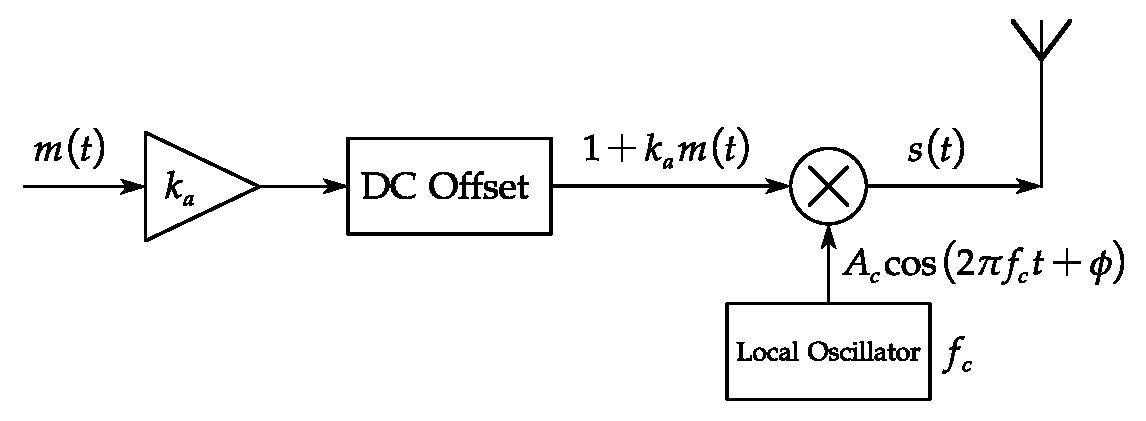
\includegraphics[scale=0.5]{plots/env_mod.pdf}
    \caption{Block diagram illustrating the process of envelope modulation.}
    \label{fig:env-mod}
\end{figure}

\subsection{Envelope Detection}
Diverging from coherent detection, envelope detection dispenses with the necessity of multiplying the received signal by the carrier wave. Instead, the received signal undergoes filtration by a Band Pass Filter (BPF) to eliminate noise beyond the desired bandwidth, and subsequently, an envelope detector facilitates the recovery of the message signal. This procedural sequence is depicted in Figure \ref{fig:env-demod}.
\begin{figure}[tb]
    \centering
    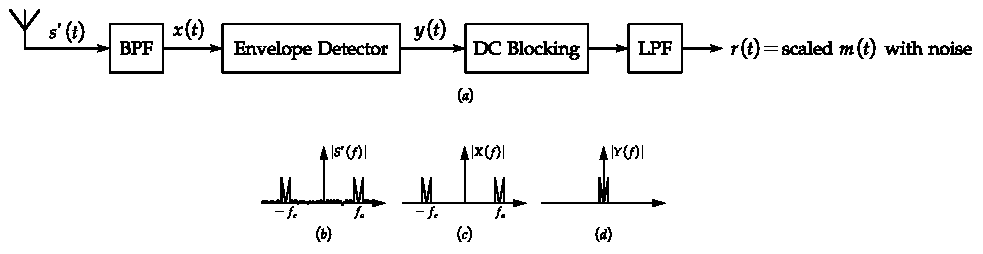
\includegraphics[width=\linewidth]{plots/env-demod.pdf}
    \caption{The envelope demodulation process. (a) The block diagram of the demodulation process. (b) The spectrum of the received noisy signal $s^\prime (t)$. (c) The spectrum of the band-pass filtered signal $x(t)$. (d) The spectrum of envelope detected signal $y(t)$.}
    \label{fig:env-demod}
\end{figure}

A common way to build the envelope detector in Python is to apply Hilbert transform \cite{ulrichEnvelopeCalculationHilbert2006, XiXiaoShengPythonTiQuXinHaoDeBaoLuoGet2023}. The envelope of an envelope-modulated signal $s\left(t\right)$ can be derived by calculating the magnitude of the Hilbert transform of the signal,
\begin{equation}
    \text{envelop of $s\left(t\right)$} = \left| \tilde{s}\left(t\right) \right|
\end{equation}
where $\tilde{s}(t)$ is the Hilbert transform of $s\left(t\right)$.

However, as is mentioned in \cite[p. 428]{kudekiAnalogSignalsSystems2009}, the Hilbert Transform is not a causal process, so is not able to be realized using analog circuits. Instead, in physical circuitry, the envelope detector typically comprises a diode and an LPF \cite{AnalogCommunicationAM}.

Figure \ref{fig:envelope} illustrates a typical diode detector circuit with a full-wave rectifier. As is discussed in \cite[pp. 111--112]{haykinIntroductionAnalogDigital2007}, on the positive segment of the signal, the diode is forward-biased and the capacitor is charged quickly. On the negative segment, the diode becomes reverse-biased and the capacitor discharges slowly through the resistor. When the input signal is greater than the output signal, the capacitor charges again; when the input signal is smaller, the capacitor discharges. In this way, the RC circuit can filter out the high-frequency carrier wave component and approximate the message signal. The time constant of the RC filter, $\tau=RC$, should satisfy
\begin{equation}
    RC\ll \frac{1}{f_c}.
\end{equation}

The charging and discharging process is visualized in Figure \ref{fig:rc-ripple} which takes a square wave as an example message signal. The output from the envelope detector is a series of saw-tooth wave that approximates the input square-wave message signal.

\begin{figure}[tb]
    \centering
    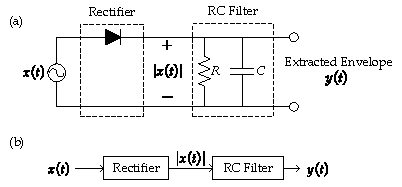
\includegraphics[scale=1.8]{plots/diode_detector.pdf}
    \caption{The diode detector. (a) The circuit of the typical diode detector. (b) The block diagram of the diode detector.}
    \label{fig:envelope}
\end{figure}
\begin{figure}[tb]
    \centering
    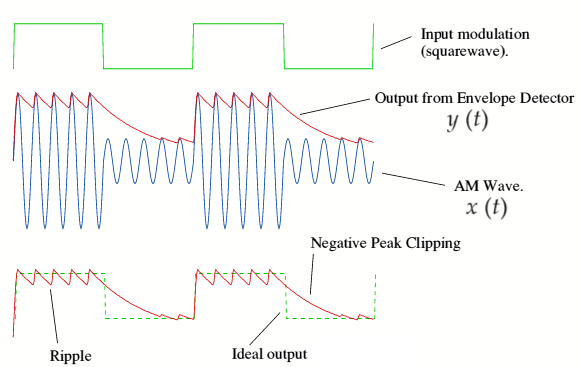
\includegraphics[width=0.7\linewidth]{plots/envelope_ripple.png}
    \caption{Ripple and peak clipping effects \cite[Fig. 9.3]{lesurfEnvelopeDetector}.}
    \label{fig:rc-ripple}
\end{figure}

\subsection{SNR Calculation and Measurement}
As is stated in \textcite[Eq. (9.26)]{haykinIntroductionAnalogDigital2007}, the theoretical pre-detection SNR in an envelope modulation receiver can be calculated by
\begin{equation}
    \SNR_{\text{pre, theoretical}}^{\text{AM}} = \frac{A_c^2 (1+k_a^2)P}{2N_0 B_T}
\end{equation}
where $A_c$ is the carrier amplitude, $k_a$ is the modulation sensitivity, $P$ is the power of message signal, $N_0$ is twice the power spectral density of white noise and $B_T$ is the noise bandwidth of the BPF.

The actual pre-detection SNR can be obtained by measuring the power of the obtained signal and that of noise. Since the filtering process will filter both the useful signal and the noise, the SNR calculation cannot simply apply the specified noise power used in AWGN generation. Instead, there are two ways of measuring the noise in this simulation:
\begin{enumerate}
    \item Calculating as the power of difference between the resulting signal under an ideal channel and that under a noisy channel.
    \item Calculating the power of noise that passes all the filters.
\end{enumerate}

Following the notation in Figure \ref{fig:env-demod}, the actual pre-detection SNR can be measured as
\begin{equation}
    \SNR_{\text{pre, measured}}^{\text{AM}} = \frac{\E[x^2(t)]}{\text{filter noise power}}.
\end{equation}
The ``filter noise power'' is measured by sending the white noise to the demodulator without any modulated signal and computing its power.

The textbook \cite[Eq. (9.23)]{haykinIntroductionAnalogDigital2007} states that the theoretical post-detection SNR in an envelope modulation receiver is expressed as
\begin{equation}
    \SNR_{\text{post, theoretical}}^{\text{AM}} = \frac{A_c^2 k_a^2 P}{2N_0 W}
\end{equation}
which is a valid approximation only for high SNR and $0<k_a<100\%$.

The actual post-detection SNR can be expressed as, if following the notation in Figure \ref{fig:env-demod},
\begin{equation}
    \SNR_{\text{post, measured}}^{\text{AM}} = \frac{\E\left[r^2(t)\right]}{\text{filter noise power}}.
\end{equation}

Theoretically, according to the calculation in \cite[Sec. 9.7]{haykinIntroductionAnalogDigital2007}, the pre- and post-detection SNR should have a relation similar to Figure \ref{fig:am-snr-theo}.
\begin{figure}[tb]
    \centering
    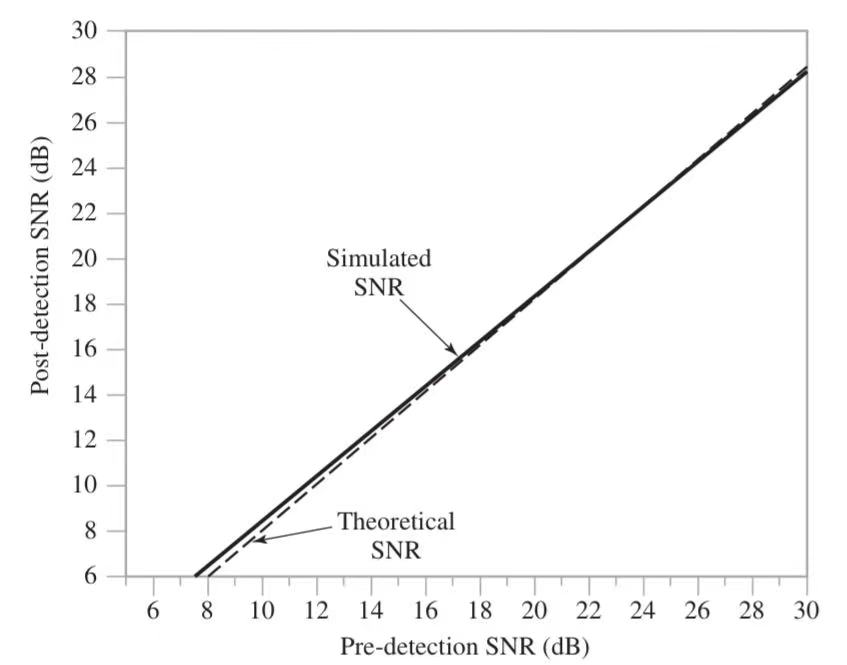
\includegraphics[width=0.5\linewidth]{plots/am_snr.jpg}
    \caption{The relation between AM pre- and post-detection SNRs \cite[Fig. 9.12]{haykinIntroductionAnalogDigital2007}.}
    \label{fig:am-snr-theo}
\end{figure}

\section{FM Simulation}
\subsection{Narrow-Band FM Modulation}
The textbook \cite[Sec. 4.1]{haykinIntroductionAnalogDigital2007} states that the message signal $m(t)$ will be phase-modulated with a carrier signal $A_c \cos\left(2\pi f_c t\right)$, which obtains the frequency modulated wave
\begin{equation}
    \label{eq:fm_modulated}
    s(t) = A_c \cos\left[ 2\pi f_c t + 2\pi k_f \int_0^{t} m\left(\tau\right) \D\tau \right]
\end{equation}
where the instantaneous frequency is
\begin{equation}
    f_i(t) = f_c + k_f m\left(t\right).
\end{equation}
Here $k_f$ denotes the modulation sensitivity which determines the frequency deviation by
\begin{equation}
    \Delta f = k_f A_m.
\end{equation}
%todo: 加上FM调制后的频谱图(应该是fc为中心,两边各延伸,范围=deviation)

By Carson's rule \cites[Sec. 4.6]{haykinIntroductionAnalogDigital2007}{CarsonRule2017}, the transmission bandwidth of an FM wave for a frequency-modulated signal is estimated as
\begin{equation}
    B_T = 2\Delta f + 2f_{m,\mathrm{max}}
\end{equation}
where $f_{m,\mathrm{max}}$ is the highest modulating frequency. The ratio of $\Delta f$ and $f_m$ is defined as modulation index,
\begin{equation}
    \beta = \frac{\Delta f}{f_m}.
\end{equation}
In this project, the modulation index is specified as $\beta=0.3$.

Such modulation can be done using a direct method \cite[Sec. 4.7]{haykinIntroductionAnalogDigital2007}, where the frequency modulator contains an oscillator directly controllable by the message signal. Figure \ref{fig:fm-mod} illustrates this process: the message signal is taken integral and sent to the controllable oscillator to produce a phase-variant signal, which is the modulated wave.
\begin{figure}[tb]
    \centering
    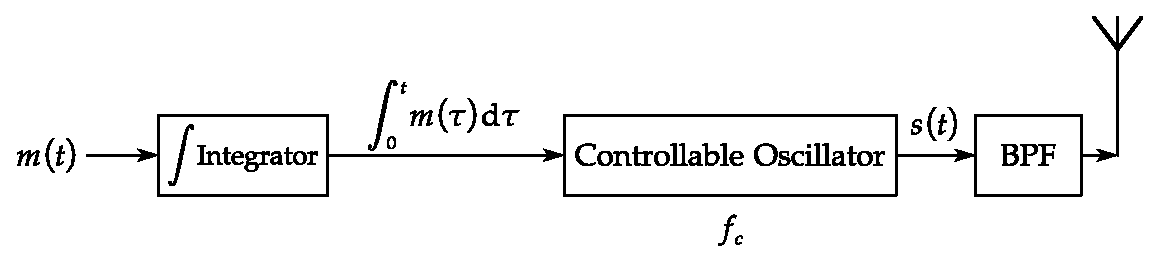
\includegraphics[scale=0.6]{plots/fm_mod.pdf}
    \caption{The direct method of narrow-band FM modulation.}
    \label{fig:fm-mod}
\end{figure}

\subsection{Narrow-Band FM Demodulation}
The key to FM demodulation is to extract the phase of the received signal. Considering an ideal channel, the received signal should equal the modulated signal $s(t)$ in Eq. \eqref{eq:fm_modulated}. Taking the derivative of $s(t)$ yields
\begin{equation}
    \nu \left( t \right) =\frac{\mathrm{d}}{\mathrm{d}t}s\left( t \right) =-A_c\left[ 2\pi f_c+2\pi k_fm\left( t \right) \right] \sin \left[ 2\pi f_ct+2\pi k_f\int_0^t{m\left( \tau \right) \mathrm{d}\tau} \right].
\end{equation}
An envelope detector could remove the sinusoidal term and get
\begin{equation}
    y\left( t \right) \approx -A_c\left[ 2\pi f_c+2\pi k_fm\left( t \right) \right]
\end{equation}
which is an approximation that only contains the scaled version of $m(t)$ and some DC offset. Hence by applying a DC blocking circuit and a proper gain to $y(t)$, the message signal can be concluded.

In practice where the channel is noisy, a BPF will be applied before differentiating and an LPF will be applied before concluding the output, both of which suppress noise introduced by the channel. The complete demodulation process is shown in Figure \ref{fig:fm-demod}.
\begin{figure}[tb]
    \centering
    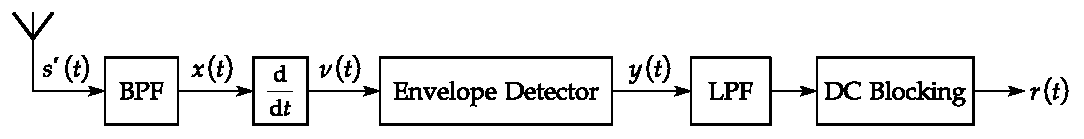
\includegraphics[scale=0.7]{plots/fm_demod.pdf}
    \caption{The demodulation process of frequency-modulated signals.}
    \label{fig:fm-demod}
\end{figure}

\subsection{SNR Calculation and Measurement}
As discussed in \cite[Sec. 9.7]{haykinIntroductionAnalogDigital2007}, the theoretical pre- and post-detection SNR is expressed as
\begin{align}
    \SNR_{\text{pre, theoretical}}^{\text{FM}} &= \frac{A_c^2}{2N_0B_T}\\
    \SNR_{\text{post, theoretical}}^{\text{FM}} &= \frac{3A_c^2 k_f^2 P}{2N_0 W}
\end{align}
where $P$ is the power of the message signal, $B_T$ is the noise bandwidth of the BPF, and $W$ is the message bandwidth. %? Relationship between B_T and W, is B_T = W? 是不是写反了

The actual SNRs can be calculated by measuring the power of the signal and noise, which can be concluded as
\begin{align}
    \SNR_{\text{pre, measured}}^{\text{FM}} &= \frac{\E\left[x^2\left(t\right)\right]}{\text{filter noise power}}\\
    \SNR_{\text{post, measured}}^{\text{FM}} &= \frac{\E[r^2(t)]}{\text{filter noise power}}.
\end{align}

Theoretically, according to the calculation in \cite[Sec. 9.8]{haykinIntroductionAnalogDigital2007}, the pre- and post-detection SNR should have a relation similar to Figure \ref{fig:fm-snr-theo} where the pre-detection SNR is linear with post-detection SNR for high pre-detection SNR.
\begin{figure}[tb]
    \centering
    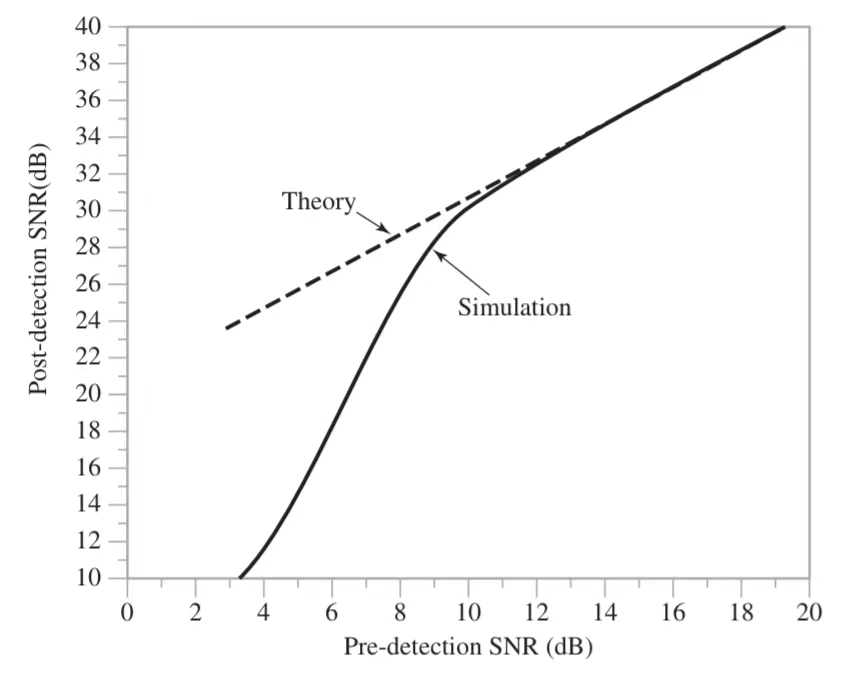
\includegraphics[width=0.5\linewidth]{plots/fm_snr.jpg}
    \caption{The relation between FM pre- and post-detection SNRs \cite[Fig. 9.17]{haykinIntroductionAnalogDigital2007}.}
    \label{fig:fm-snr-theo}
\end{figure}


\section{Filter Design}
\subsection{Ideal Filters}
The filters remove the unnecessary frequency components of its input signals. Figure \ref{fig:ideal-filter} shows the impulse response of an ideal LPF and BPF.

The expressions for ideal LPF and BPF in the frequency domain are
\begin{align}
    H_{LPF}\left(f\right) &= \rect\left( \frac{f}{2f_{cut}} \right) \\
    H_{BPF}\left(f\right) &= \rect\left( \frac{f-f_{cut}}{2f_{cut}} \right) + \rect\left( \frac{f+f_{cut}}{2f_{cut}} \right)
\end{align}
By inverse Fourier transformation, their time-domain impulse response can be obtained as
\begin{align}
    h_{LPF}\left(t\right) &= 2f_{cut}\sinc\left(2f_{cut} t\right) \\
    h_{BPF}\left(t\right) &= 2f_{cut}\sinc\left(2f_{cut} t\right)\e^{j2\pi f_{cut} t} + 2f_{cut}\sinc\left(+2f_{cut} t\right)\e^{-j2\pi f_{cut} t}
\end{align}
which contains non-periodic and infinitely expanding $\sinc$ terms. This indicates the impulse response to be associated with the future input, which violates the causality. Thus the ideal LPF and BPF are not causal and are not physically implementable.

\begin{figure}[tb]
    \centering
    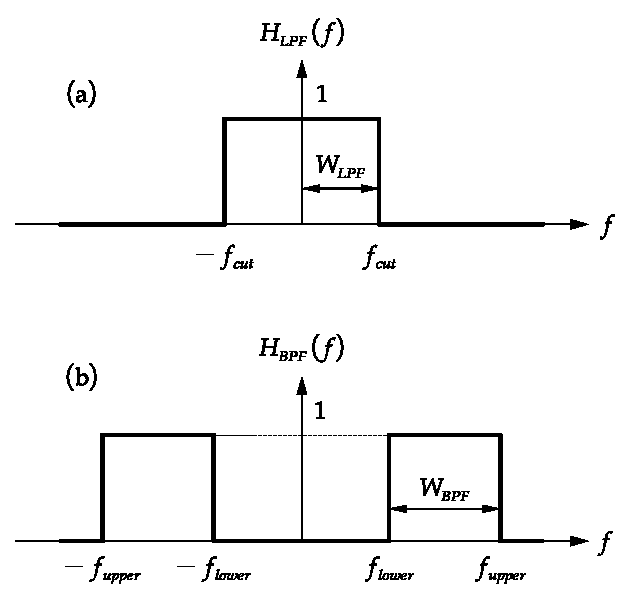
\includegraphics[scale=0.6]{plots/ideal-filters.pdf}
    \caption{The impulse response of ideal LPF and BPF. (a) The impulse response of an ideal LPF. $W_{LPF}$ shows the bandwidth of the LPF. (b) The impulse response of an ideal BPF. $W_{BPF}$ shows the bandwidth of the BPF.}
    \label{fig:ideal-filter}
\end{figure}

\subsection{Butterworth Filter in Python}

Both Amplitude Modulation (AM) and Frequency Modulation (FM) communication systems necessitate the incorporation of filters. In practical scenarios, however, the realization of ideal filters poses inherent challenges. Nevertheless, the Butterworth Filter exhibits characteristics closely approximating those of an ideal filter. Figure \ref{fig:butter-ckt} illustrates an analog circuit design of a first-order Butterworth LPF which is composed of an operational amplifier. According to \cite{ButterworthFilterWhat2021}, the general $n$-th order Butterworth LPF has a transfer function
\begin{equation}
    H_{n}\left( j\omega \right) =\frac{1}{\sqrt{1+\epsilon ^2\left( \frac{\omega}{\omega _c} \right) ^{2n}}}
\end{equation}
where $\epsilon$ is the maximum pass-band gain and $\omega_c$ is the cut-off frequency. Figures \ref{fig:butter-lpf} and \ref{fig:butter-bpf} depict the frequency responses of Butterworth LPF and BPF with varying orders, illustrating that an increased order ($n$) results in a more pronounced roll-off slope. As expounded by \cite{storrButterworthFilterDesign2013, kudekiAnalogSignalsSystems2009}, a Butterworth Low Pass Filter manifests a maximally flat frequency response within its passband, swiftly attenuating beyond the cut-off frequency. This advantageous attribute empowers the design of filters with minimal distortion, albeit at the expense of an indeterminate phase delay induced by the inherent properties of Infinite Impulse Response (IIR) filters.

In the digital realm, Python facilitates the implementation of filters as digital IIR filters, with each filter in the $z$-domain expressed as the quotient of two polynomials:
\begin{equation}
    H_{\text{digital}}(z) = \frac{\sum_{p=0}^{n}{a_pz^{-p}}}{\sum_{q=0}^{n}{b_qz^{-q}}}.
\end{equation}

The response of the filter is uniquely determined by coefficients $a_i$ and $b_j$ ($0 \leq i, j \leq n$), where these coefficients can be computed using the \verb|scipy.signal.butter()| function, as documented by \cite{thescipycommunityScipySignalButter, thescipycommunityScipySignalFiltfilt, thescipycommunityScipySignalLfilter}.

\begin{figure}[tb]
    \centering
    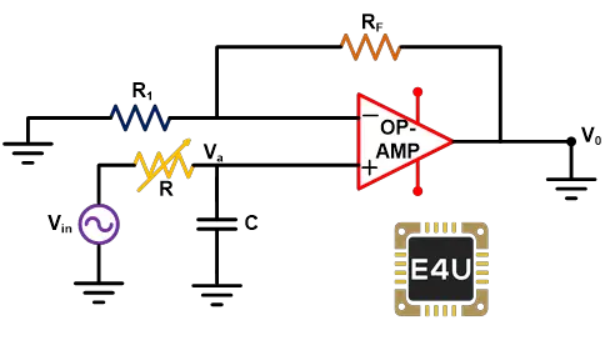
\includegraphics[scale=.5]{plots/1order_butterLPF.png}
    \caption{A first-order Butterworth LPF circuit \cite{ButterworthFilterWhat2021}.}
    \label{fig:butter-ckt}
\end{figure}
\begin{figure}[tb]
    \centering
    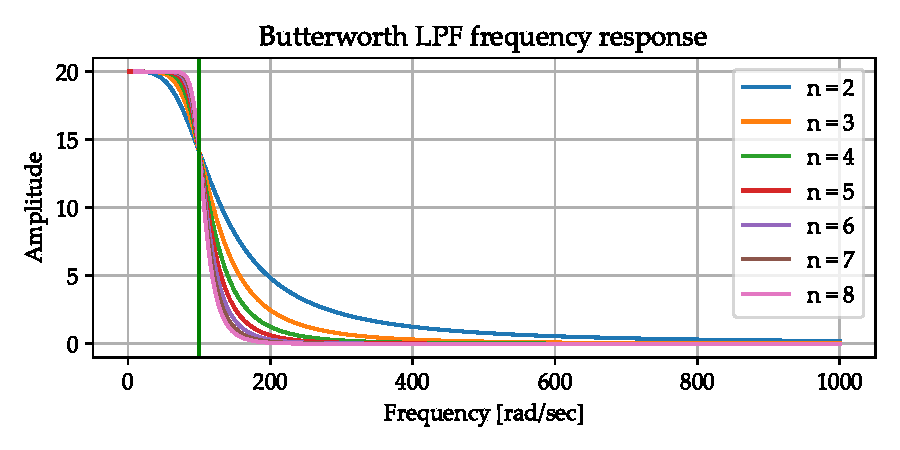
\includegraphics[scale=.8]{plots/butterworth-lpf-nolog.pdf}
    \caption{The frequency response of a Butterworth LPF with cut-off frequency $\omega_c = \SI{100}{\radian\per\s}$.}
    \label{fig:butter-lpf}
\end{figure}
\begin{figure}[tb]
    \centering
    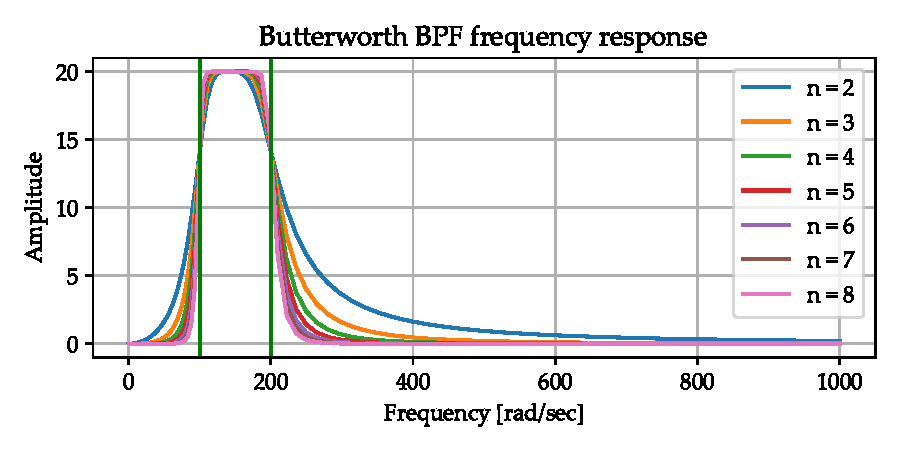
\includegraphics[scale=.8]{plots/butterworth-bpf-nolog.pdf}
    \caption{The frequency response of a Butterworth BPF with pass-band from \SI{100}{Hz} to \SI{200}{Hz}.}
    \label{fig:butter-bpf}
\end{figure}

\subsection{Nyquist Sampling Theorem}

The sampling frequency is of significance in the design of the Butterworth filter. As stated in \cite[pp. 296--297]{manolakisAppliedDigitalSignal2011}, the sampling frequency $f_s$ should satisfy
\begin{equation}
    f_s \geq 2B_W
\end{equation}
where $B_W$ is the bandwidth of the signal to sample. Hence in filter design, the frequency parameters should also follow the sampling theorem,
\begin{align}
    f_{cut, LPF} &\leq \frac{f_s}{2} \\
    f_{lower, BPF}&< f_{upper, BPF}\leq \frac{f_s}{2}.
\end{align}

\end{document}